% Figura cuerpo B1: de dónde viene la nueva macroeconomía clásica, en qué se divide y qué deja (temas 3.A.4 a 3.A.7)
\documentclass[tikz,border=3pt]{standalone}
\usepackage[T1]{fontenc}
\usepackage[utf8]{inputenc}
\usetikzlibrary{arrows.meta,calc,positioning}
\begin{document}
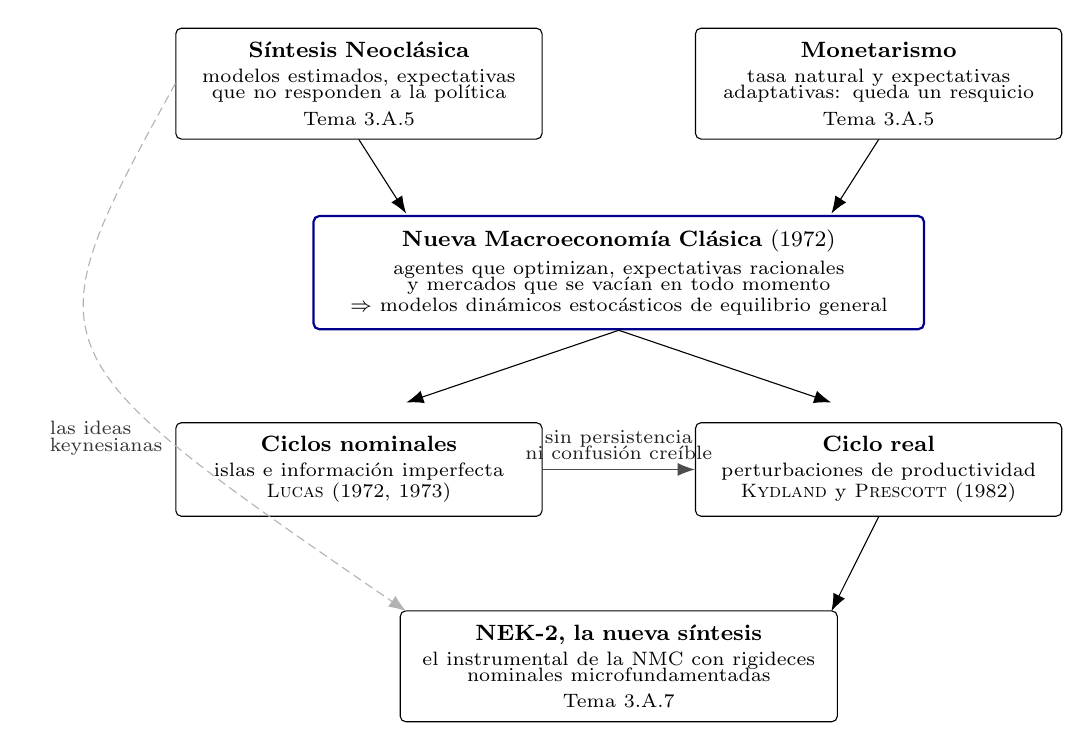
\begin{tikzpicture}[>={Latex[length=2.2mm]}, line cap=round, font=\footnotesize,
  caja/.style={draw, rounded corners=2pt, align=center, inner sep=5pt},
  azul/.style={draw=blue!55!black, thick, rounded corners=2pt, align=center, inner sep=5pt},
  gris/.style={draw=gray!60, rounded corners=2pt, align=center, inner sep=4pt, font=\scriptsize, text=gray!25!black}]
  % Herencia
  \node[caja, text width=4.3cm] (snc) at (2.6,5.4) {\textbf{Síntesis Neoclásica}\\[1pt]\scriptsize modelos estimados, expectativas\\[-2pt]\scriptsize que no responden a la política\\\scriptsize Tema 3.A.5};
  \node[caja, text width=4.3cm] (mon) at (9.2,5.4) {\textbf{Monetarismo}\\[1pt]\scriptsize tasa natural y expectativas\\[-2pt]\scriptsize adaptativas: queda un resquicio\\\scriptsize Tema 3.A.5};
  % Nucleo
  \node[azul, text width=7.4cm] (nmc) at (5.9,3.0) {\textbf{Nueva Macroeconomía Clásica} (1972)\\[2pt]\scriptsize agentes que optimizan, expectativas racionales\\[-2pt]\scriptsize y mercados que se vacían en todo momento\\[-2pt]\scriptsize $\Rightarrow$ modelos dinámicos estocásticos de equilibrio general};
  \draw[->] (snc.south) -- (3.2,3.75);
  \draw[->] (mon.south) -- (8.6,3.75);
  % Dos motores
  \node[caja, text width=4.3cm] (islas) at (2.6,0.5) {\textbf{Ciclos nominales}\\[1pt]\scriptsize islas e información imperfecta\\[-2pt]\scriptsize \textsc{Lucas} (1972, 1973)};
  \node[caja, text width=4.3cm] (rbc) at (9.2,0.5) {\textbf{Ciclo real}\\[1pt]\scriptsize perturbaciones de productividad\\[-2pt]\scriptsize \textsc{Kydland} y \textsc{Prescott} (1982)};
  \draw[->] (nmc.south) -- (3.2,1.35);
  \draw[->] (nmc.south) -- (8.6,1.35);
  \draw[->, gray!60!black] (islas.east) -- (rbc.west) node[midway, above, font=\scriptsize, text=gray!25!black, align=center]{sin persistencia\\[-2pt]ni confusión creíble};
  % Herencia posterior
  \node[caja, text width=5.2cm] (nek) at (5.9,-2.0) {\textbf{NEK-2, la nueva síntesis}\\[1pt]\scriptsize el instrumental de la NMC con rigideces\\[-2pt]\scriptsize nominales microfundamentadas\\\scriptsize Tema 3.A.7};
  \draw[->] (rbc.south) -- (8.6,-1.3);
  \draw[->, densely dashed, gray!60] (snc.west) ..controls (-1.6,2.0).. (3.2,-1.3);
  \node[gray!40!black, font=\scriptsize, anchor=west, align=left] at (-1.45,0.9) {\scriptsize las ideas\\[-2pt]\scriptsize keynesianas};
\end{tikzpicture}
\end{document}
